\documentclass[conference, 5pt]{IEEEtran}

\usepackage{amsmath}
\usepackage{graphicx}
\usepackage{todonotes}
\usepackage[inline]{enumitem}
\usepackage{xcolor}
\usepackage{subcaption}
\graphicspath{{./figures/}}
\begin{document}
\title{The Information Bottleneck for Deep Schizophrenia Classification}
\renewcommand{\todo}[1]{\color{red}{#1}\color{black}}
\author{
\IEEEauthorblockN{Brandon Boos}
\IEEEauthorblockA{University of New Mexico\\
btboos@unm.edu}
\and
\IEEEauthorblockN{Brad Baker}
\IEEEauthorblockA{The Mind Research Network\\University of New Mexico\\bbaker@mrn.org}}

% make the title area
\maketitle

% no keywords

\IEEEpeerreviewmaketitle

\section{Introduction}

Deep Neural Networks (DNNs) as a class of machine-learning model have seen a wide breadth of applications in various problem domains. Despite this prevalence of application, there is little theoretical understanding for how the various components of DNNs aid in the overall learning of complex, non-linear relationships. In an attempt to bridge this gap, a recent paper from Shwartz Et. al. proposed an information-theoretic interpretation of DNNs, based on the so-called Information-Bottleneck \cite{shwartz2017opening} method, a method which provides a theoretical framework for describing the optimal trade-off between the compression of input features $X$ and the prediction of output labels $Y$ \cite{tishby2000information}. Using this method as part of a larger information-theoretic analysis of DNNs, Shwartz et. al. argue for three main findings: 
\begin{enumerate*}
\item DNNs with stochastic-gradient optimization undergo two distinct phases of information increase around input labels (fitting), and decrease around input features (relaxation) which amounts to a maximization of the conditional entropy of the DNNs layers subject to an empirical error constraint,
\item  learned layers lie very closed to the Information-Bottleneck Bound \cite{tishby2000information}, and satisfy Information-Bottleneck optimality (i.e. they maximize the optimal trade-off between compression of input features and prediction of output labels)
\item finally, the advantage of including hidden layers in DNNs is mostly computational, with these hidden layers providing faster convergence times towards this maximization of conditional entropy of the layers.
\end{enumerate*}\cite{shwartz2017opening}

Though this interpretation of DNNs has recently sparked controversy \cite{saxe2018information,amjad2018information}, We propose a project which examines this information-theoretic interpretation of DNNs for one particular task in neuro-imaging analysis: classification of schizophrenia data. Classification of schizophrenia patients with neuroimaging data is one problem in neuroimaging which has recently seen initial success with DNNs \cite{plis2014deep,kim2016deep,han2017schizophrenia}; however, no theoretical interpretation exists for how the utilized DNNs leverage this data to perform the classification task. We believe that an investigation in the style of Shwartz et. al. 2017 \cite{shwartz2017opening} could provide initial steps towards such an explanation. 

``First, at a high level, I would argue that Neural Networks themselves are examples of Complex Adaptive Systems. The non-linear interactions between the neurons underpin the emergent, complex computational behavior of the Neural Network as a whole, and as of yet, there is no accepted theoretical framework for explaining exactly how this lower-to-higher level organization works. As a consequence, there exists no theoretical explanation surrounding how Neural Networks and the underlying optimization procedures as systems utilize information to answer problems like image classification. 

Schwartz et al. 2017 argues for an Information-Theoretic explanation of Neural Networks and their constituent components. Their level of granularity stays at the level of layer-wise and optimization-based analyses, rather than interactions between individual neurons; however, I would argue that this is just a matter of looking at different levels of organization (e.g. looking at functionally distinct regions of the brain vs. looking at individual neurons). The first of the Schwartz hypotheses argue for two distinct phases of information-processing within the layers, as we described in the paper, where layers learn first to represent the labels, and second to represent the features, in a hierarchical fashion (deeper layers typically having higher information), as the network as a whole converges toward an optimal representation for predicting labels, given the input features. 

The second hypothesis describes layer-wise and global convergence towards this Information-Bottleneck bound, with the underlying idea being that the layers approach this boundary by in a theoretical sense, moving through this "information-plane" (where coordinates are given in terms of information around the labels (Y-axis) and features (X-axis) ). Again, this is a method for describing how information changes in the layers individually, but also in the neural network as a whole, with the Information-Bottleneck bound used as an indicator for the system's ability to compute the given problem (classification).

The hypothesis regarding additional deep layers is an argument about how the additional of additional constituent parts (layers) contributes to the system's ability to converge toward this Information-Bottleneck bound (and thus converge to the classification). Their assertion is that the addition of further layers allows the deeper layers to reach the optimum with fewer epochs. In more Complex Adaptive Systems terms, the addition of further agents (layers), increases the computational speed at which the system as a whole is able to perform the given problem (classification). That deeper layers lead to better generalization in less epochs in DNNs is an intuition widely held in the DNN community, I believe, though of course it can add additional problematic issues, such as increase in run-time due to back-propagation over the additional parameters, or over-fitting on training features.

To summarize, our project amounts to an extension of the empirical investigation for a particular information-theoretic explanation within on Complex Adaptive System (DNNs). We examine both the empirical results for changes to hyper parameters (either architecture or optimization parameters, both if we have enough time), and explore the application for a familiar problem for a new data modality.''

\subsection{Contributions}

\begin{enumerate}
	\item An extended view of the effect of Hyper-Parameters on the Information-Plane through the analysis of 
    	\begin{enumerate}
        	\item The Learning Rate
            \item L1, L2, and Elastic-Net Regularization
            \item 7 Different Activation Functions (TanH, Sigmoid, ReLU, SoftPlus, )
        \end{enumerate}
    \item An initial analysis of the Information-Plane and Information-Bottleneck Dynamics of Several Deep Neural Network architectures used for classifying three Schizophrenia Data Sets.
\end{enumerate}

\section{Methods}

For all of our analyses, we utilize the tools provided on GitHub by the authors of \cite{shwartz2017opening}.  For each tested DNN, we treat each of the layers $1\le i\le K$ in the network as a single variable $T_i$ and compute the mutual information between each layer with the input and with the labels. To do this, each layer's neuronal activation is binned into 30 equal intervals in $[-1, 1]$, and the joint distributions $P(T_i,X)$ and $P(T_i,Y)$ are estimated as in \cite{shwartz2017opening}.

\subsection{The Information-Plane View of Hyper-Parameters}

We first extend the analysis in \cite{shwartz2017opening} by taking a look at how the changes in SGD optimization hyper parameters change the information-plane dynamics of a given DNN. For the purpose of our analysis we focus on three classes of hyper-parameter: the Learning Rate, Regularization Parameters, and the Activation functions. In complex adaptive system terms, this analysis amounts to a changing of the structure of the underlying complex model, where the learning rate and regularization terms operate on the scale of the global optimization, and the activation function operates on the scale of individual neurons. 

To compare more directly with the results in \cite{shwartz2017opening}, we utilize the provided numerical data created by the authors of \cite{shwartz2017opening}.



\subsection{The Information-Plane View of Schizophrenia Classification}

In this section, we 

\section{Results}

\subsection{The Information-Plane view of Hyper-Parameters}

\begin{figure*}
	\begin{subfigure}{0.32\linewidth}
    \label{fig:tanh_activation}
	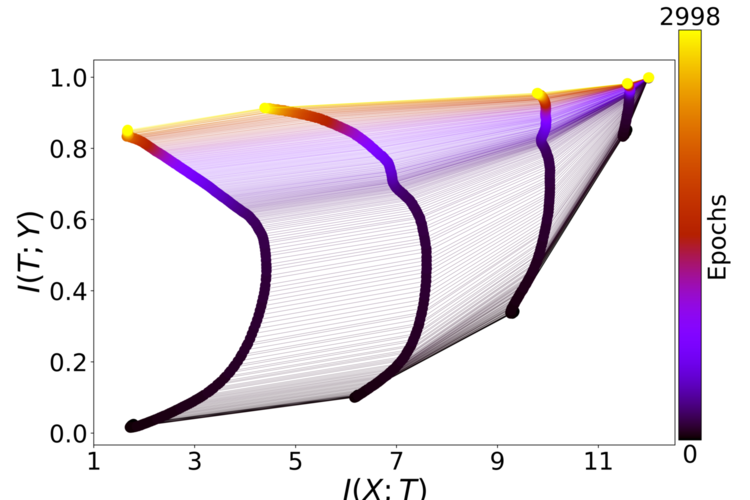
\includegraphics[width=\columnwidth]{activations/tanh.png}
    \subcaption{tanh}
    \end{subfigure}
    	\begin{subfigure}{0.32\linewidth}
    \label{fig:elu_activation}
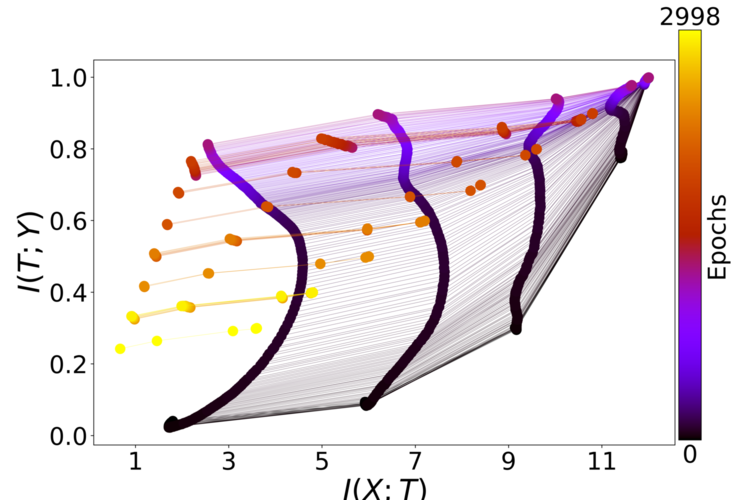
\includegraphics[width=\columnwidth]{activations/elu.png}
   \subcaption{elu}
\end{subfigure}
    	\begin{subfigure}{0.32\linewidth}
    \label{fig:sigmoid_activation}
	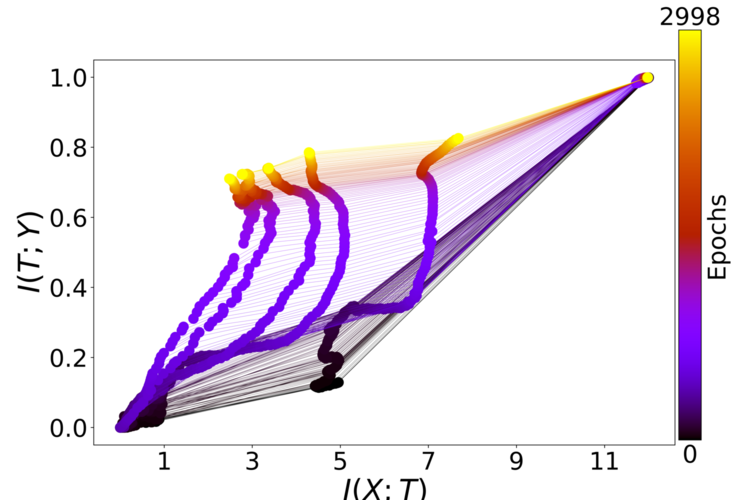
\includegraphics[width=\columnwidth]{activations/sigmoid.png}
   \subcaption{sigmoid}
\end{subfigure}
        	\begin{subfigure}{0.32\linewidth}
    \label{fig:sp_activation}
	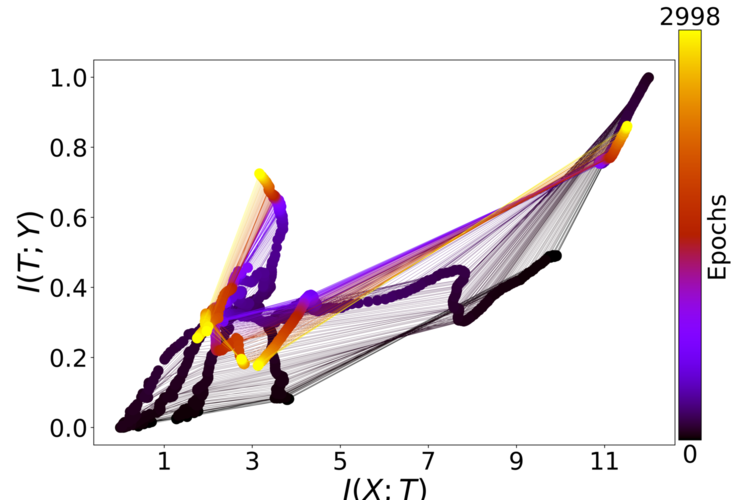
\includegraphics[width=\columnwidth]{activations/softplus.png}
   \subcaption{softplus}
\end{subfigure}
        	\begin{subfigure}{0.32\linewidth}
    \label{fig:ss_activation}
	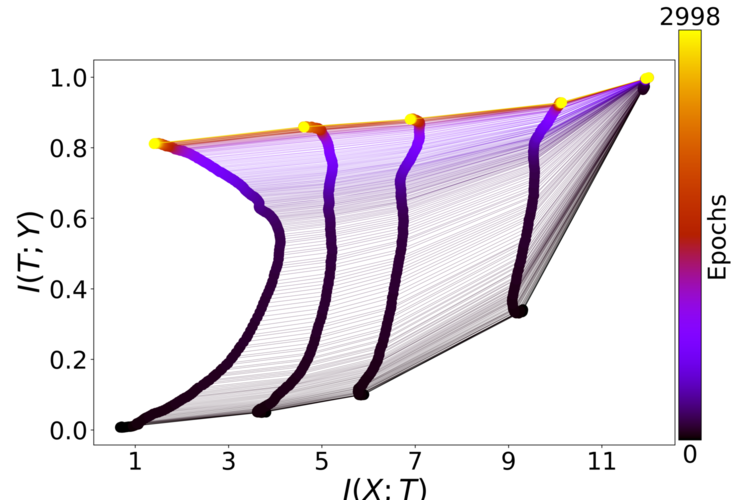
\includegraphics[width=\columnwidth]{activations/softsign.png}
   \subcaption{softsign}
\end{subfigure}
        	\begin{subfigure}{0.32\linewidth}
    \label{fig:lsm_activation}
	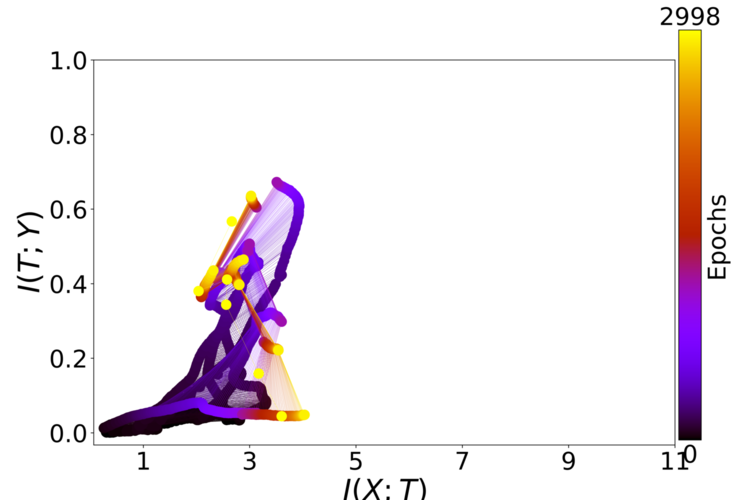
\includegraphics[width=\columnwidth]{activations/log_softmax.png}
   \subcaption{log softmax}
\end{subfigure}
\end{figure*}

\begin{figure*}
	\begin{subfigure}{0.25\linewidth}
		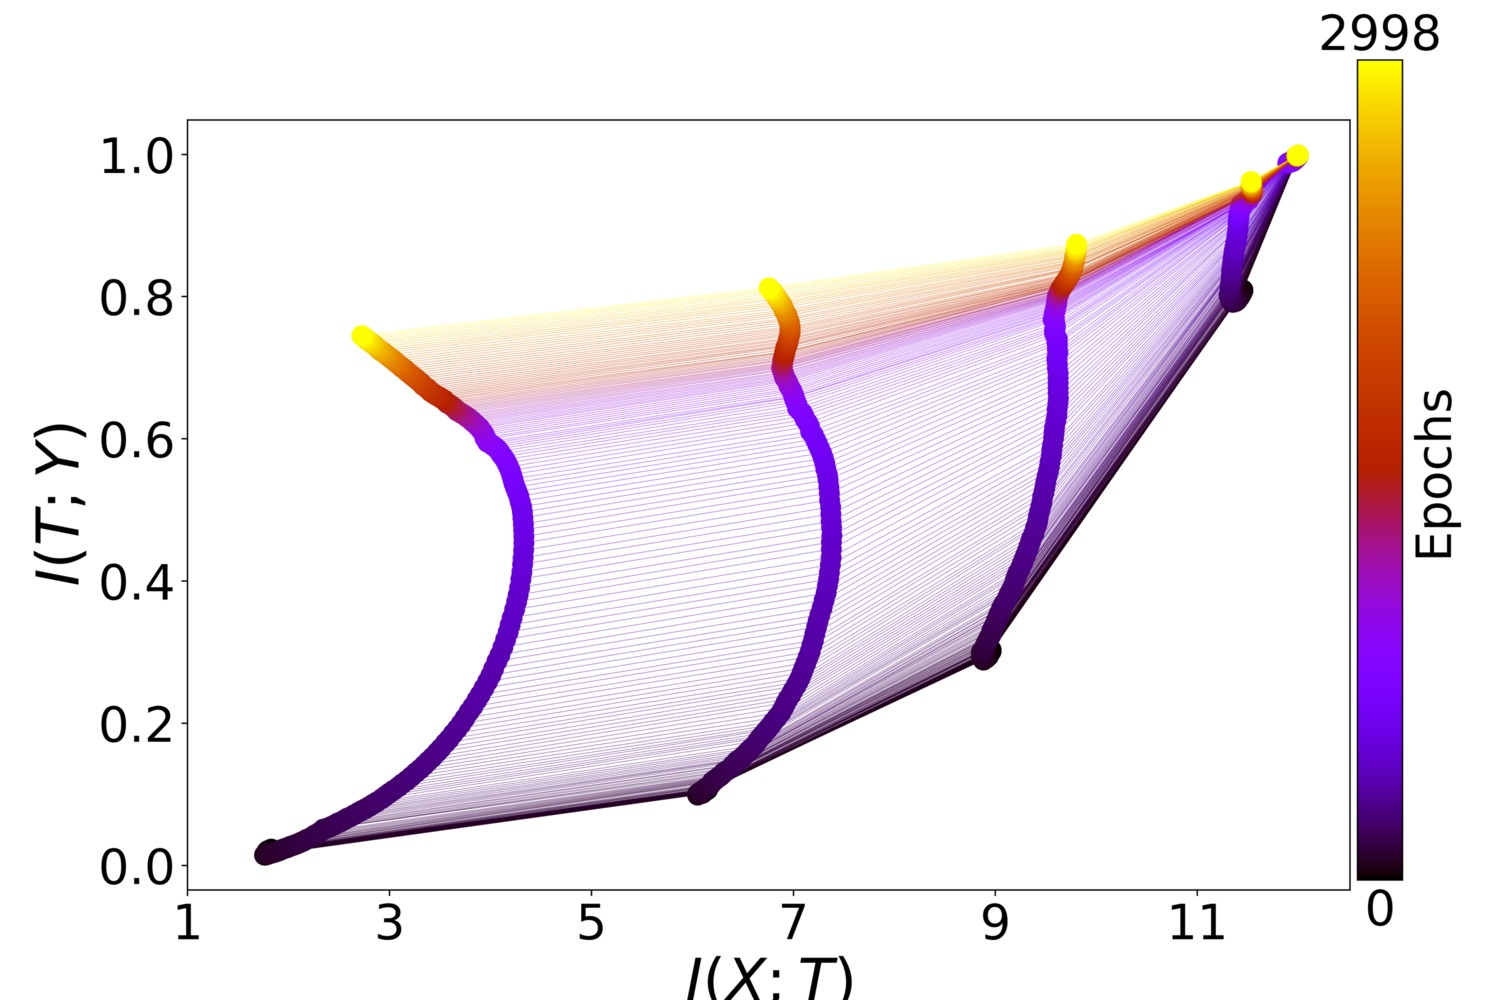
\includegraphics[width=\columnwidth]{search/lr0_0001.png}
	\end{subfigure}
    \begin{subfigure}{0.25\linewidth}
		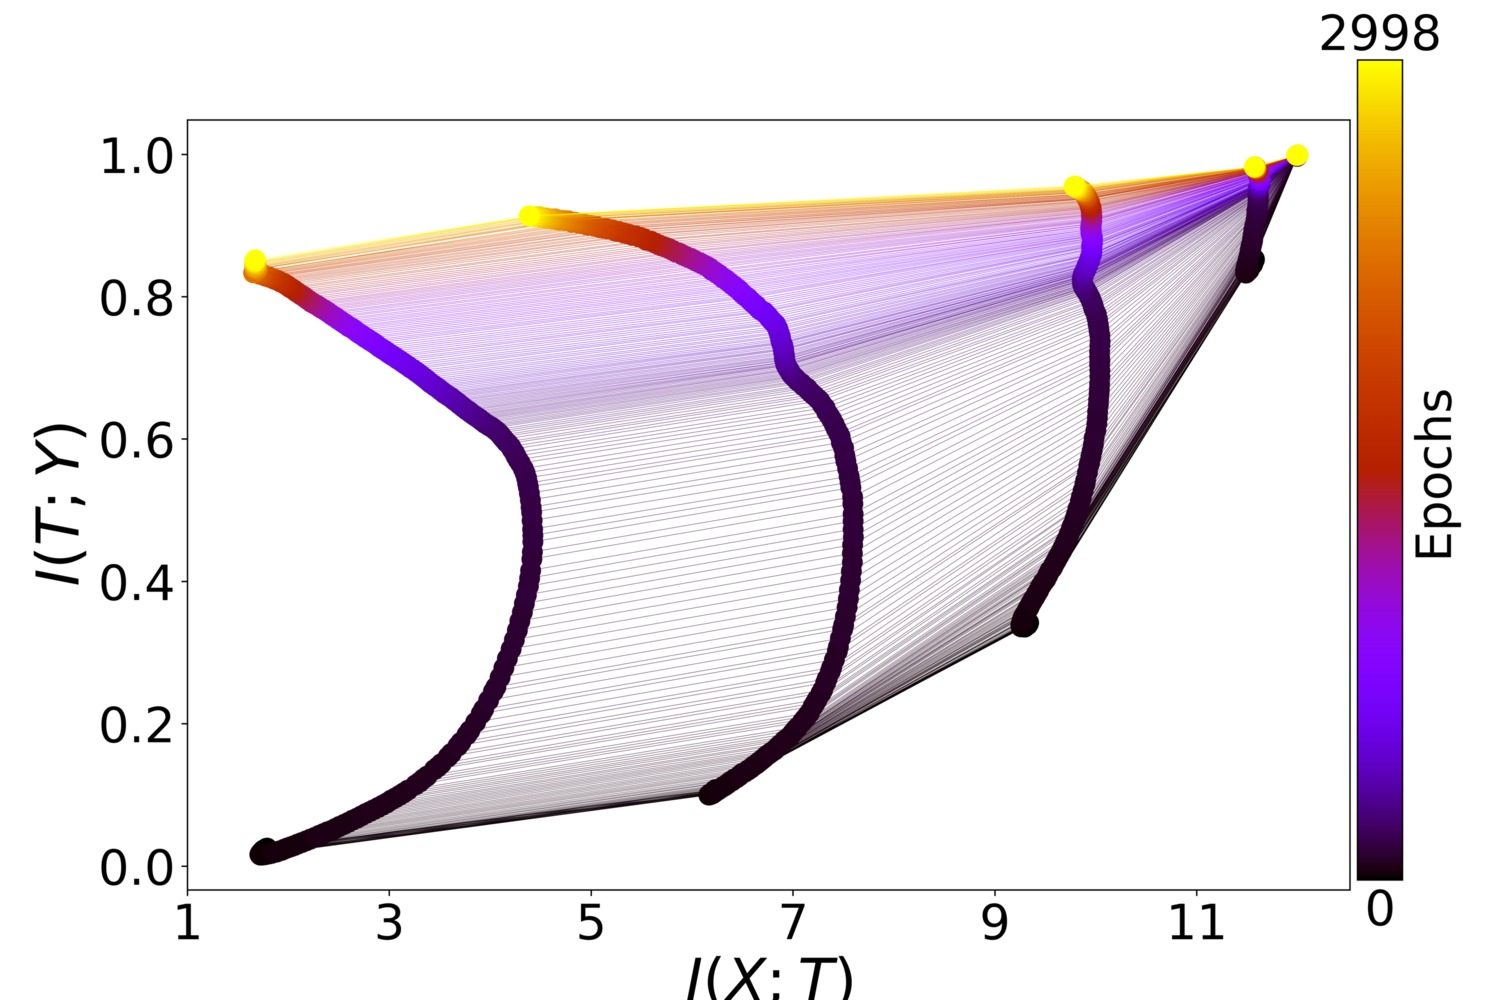
\includegraphics[width=\columnwidth]{search/lr0_0004.png}
	\end{subfigure}
    \begin{subfigure}{0.25\linewidth}
		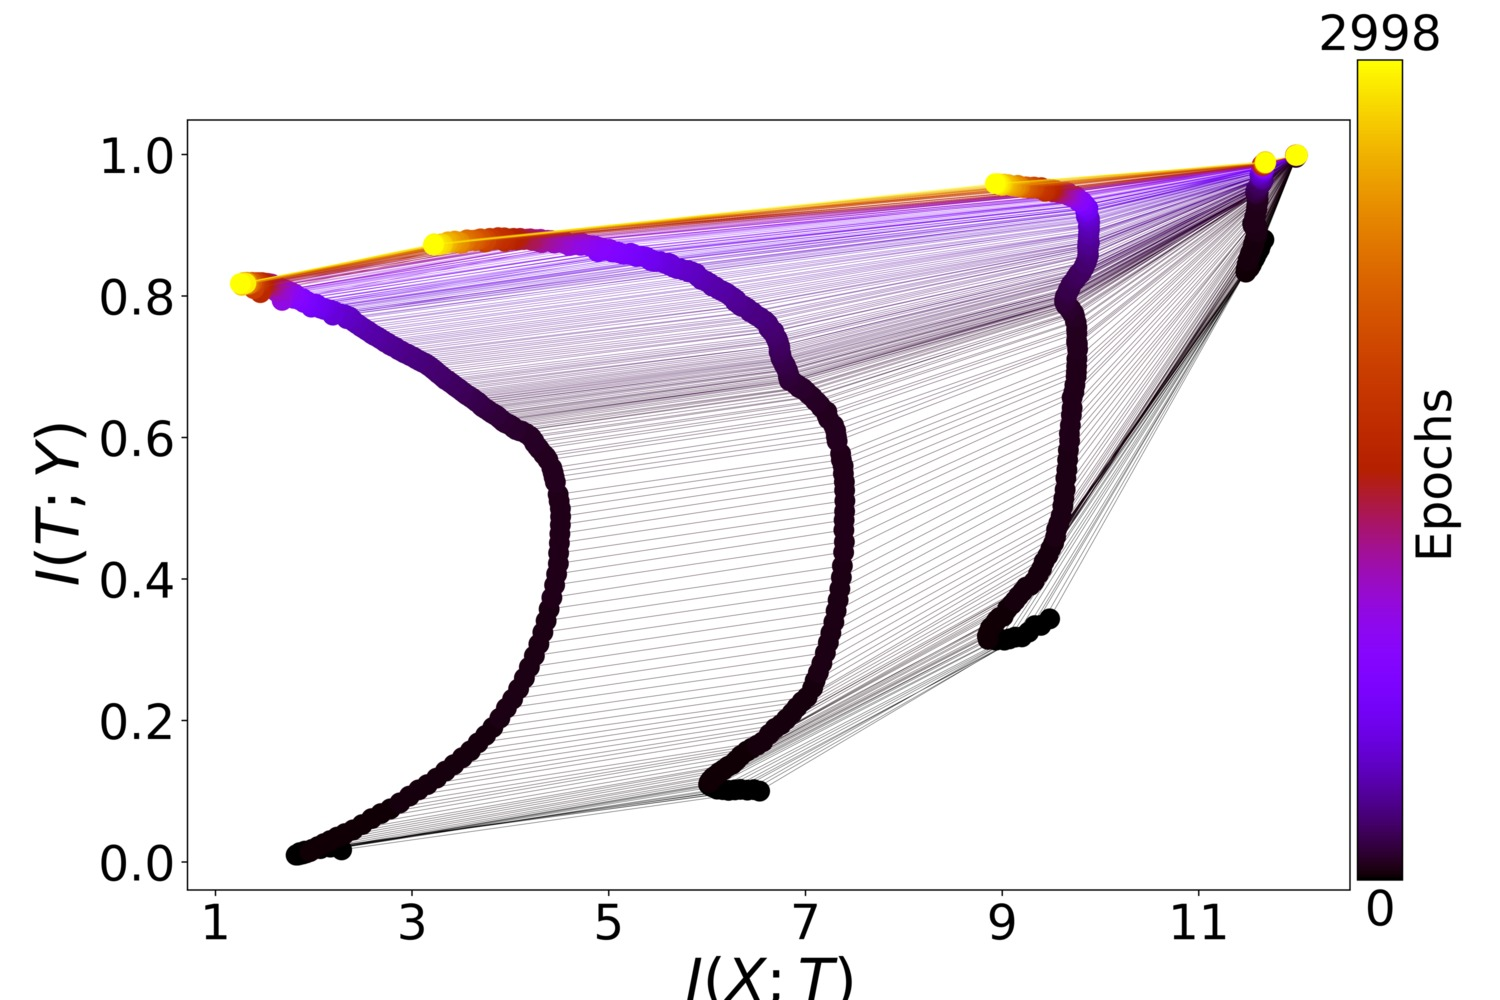
\includegraphics[width=\columnwidth]{search/lr0_0010.png}
	\end{subfigure}
\end{figure*}

\subsection{The Information-Plane View of Schizophrenia Classification}


\begin{figure}
\caption{An information-based figure for Hyper-Parameters based off figure 5, for learning rate and l1 regularization}
\end{figure}

\subsection{NeuroImaging Data}

\begin{figure}
\caption{Animation of 50 repeated runs for neuroimaging data}
\end{figure}

\begin{figure}
\caption{Loss for training Neuroimaging}
\end{figure}

\begin{figure}
\caption{Information Plane figure for Neuroimaging data}
\end{figure}

\section{Discussion}


\section{Conclusion}

\cite{shwartz2017opening}

\bibliography{project_3}
\bibliographystyle{IEEEtran}


% that's all folks
\end{document}



